\documentclass[10pt,a4paper,twocolumn]{article}
\usepackage[T1]{fontenc}
\usepackage[sc]{mathpazo}
\usepackage[margin=19mm]{geometry}
\usepackage{microtype,amsmath,amssymb,amsthm,graphicx,booktabs}
\usepackage{algorithm,algpseudocode}
\usepackage{xcolor}
\definecolor{ProjectBlue}{HTML}{174F91}
\usepackage[colorlinks=true,allcolors=ProjectBlue,
  pdftitle={Seven-Day AI Forecasts for German Hydrogen Reserve Operations},
  pdfauthor={Parsa Besharat}]{hyperref}
\setlength{\columnsep}{7mm}
\setlength{\emergencystretch}{1em}
\raggedbottom
\newcommand{\repo}{\href{https://github.com/parsabe/Beyond-Normal-Weather/tree/germany-ai-operations/germany}{Germany pipeline repository}}
\title{Seven-Day AI Forecasts for German Hydrogen Reserve Operations}
\author{Parsa Besharat\\\normalsize\href{mailto:parsa@parsabe.com}{\texttt{parsa@parsabe.com}}}
\date{}

\begin{document}
\maketitle

\begin{abstract}
Reliable industrial hydrogen delivery depends on how operators respond to multi-day wind and solar shortages. This pilot forecasts daily renewable generation across Germany's four electricity control areas using a neural network trained on historical generation and archived weather forecasts. It compares standard training and training that gives greater weight to windows of low modeled hydrogen supply. Each forecast is expanded into eight correlated weekly scenarios and passed to a rolling linear optimizer that recommends regional reserve targets and backup import orders. The evaluation replays 359 historical decision days and compares the policies with linear forecasting, persistence, and a fixed reserve rule. Ridge regression gave the lowest forecast error. During a modeled import interruption, the reserve-weighted neural policy improved on the ordinary neural policy, while the fixed reserve rule missed the fewest deliveries. The \repo\ contains the configuration, code, and results for the illustrative supply system.
\end{abstract}

\section{Introduction}
Germany's hydrogen strategy identifies diversification of energy imports and security of supply as priorities \cite{strategy}. For operators with renewable power contracts, backup supply and stored hydrogen offer flexibility when wind and solar generation fall. Reserve decisions depend on how long shortages are expected to last and whether several regions are exposed at once. Germany's four control areas provide a useful geographic division for studying this question with public generation data. This pilot asks whether a neural estimate of next-week renewable supply helps an illustrative four-zone portfolio decide how much hydrogen to reserve and which zones need backup orders. Its criterion is delivery performance under the same physical and contractual assumptions across all forecasting methods.

\section{Related Work}
Research on German \emph{Dunkelflauten} connects multi-day low renewable generation to winter weather regimes \cite{mockert}. Probabilistic renewable forecasts have also been used for stochastic control of wind--solar hydrogen systems \cite{mpc}. The question here is whether joint regional forecasts and greater training weight on low-supply windows help reserve decisions under a common optimizer and independently held-out historical data. Delivery and cost estimates are specific to the tested configuration.

\section{Methodology}
\subsection{Learning regional renewable trajectories}
The target is a seven-day matrix of observed wind and solar generation in 50Hertz, Amprion, TenneT, and TransnetBW. SMARD supplies daily generation \cite{smard}. Predictors include recent generation up to two days before issue, seasonal terms, and archived ECMWF wind speed and solar radiation from Open-Meteo at two points per zone \cite{meteo}. The weather features use the appropriate preceding-day offset for each target date and retain local valid hours through 18:00. This creates a time buffer relative to the decision hour. The archive provides lead offsets rather than an exact release timestamp for every value.

A fully connected neural network with hidden layers of 64 and 32 units predicts the entire matrix. One fit uses squared error, and a second triples the sample weight of the weakest fifth of training windows. Weak supply is defined as the lowest three-day mean of national modeled hydrogen production potential within a week. A ridge model uses identical inputs. Persistence repeats the latest generation available to the forecaster. Forecasts are clipped at zero. Whole residual trajectories from the calibration interval are sampled according to season and expected renewable supply. Adding a whole trajectory preserves cross-zone and cross-day errors within each draw.

\subsection{Reserve and import decisions}
For zone $z$, day $t$, and forecast scenario $s$, the dispatch model balances storage according to
\begin{equation}
\label{eq:balance}
S_{s,t,z}=S_{s,t-1,z}+P_{s,t,z}+I_{s,t,z}
+F^{\mathrm{net}}_{s,t,z}-D_z+U_{s,t,z}.
\end{equation}
Here $P$ is local production, $I$ is backup hydrogen, $D$ is contracted demand, $U$ is unmet demand, and $F^{\mathrm{net}}$ is incoming minus outgoing transfer. Production, inventories, imports, and transfers have upper limits. Today's import orders are shared across scenarios. The objective combines expected operating costs, unmet demand penalties, a penalty for falling below the terminal stock target, and conditional value at risk of cumulative shortage. With eight equal paths and a 90\% tail level, that last term emphasizes the worst sampled shortage. The end-of-day reserve recommendation is the scenario average of planned stocks. For evaluated operations, day-ahead orders are fixed and a daily recourse calculation uses realized generation.

\begin{algorithm}[t]
\caption{Rolling reserve recommendation and replay}
\small
\begin{algorithmic}[1]
\State Train the renewable models on the training interval.
\State Save calibration errors as full weekly trajectories.
\For{each held-out issue day}
  \State Predict seven days of generation by zone and type.
  \State Draw eight scenarios from comparable weekly errors.
  \State Solve for today's shared orders and stock targets.
  \State Fix orders and replay dispatch at realized supply.
  \State Carry closing reserves into the following day.
\EndFor
\end{algorithmic}
\end{algorithm}

\section{Experiments}
The study trains in April--December 2024, calibrates in January--September 2025, and evaluates 359 daily issues from 1 October 2025 to 24 September 2026. Each seven-day window ends within its split. Daily winds and solar observations cover Germany's four control areas. Capacities, costs, contracted renewable shares, and hydrogen links are defined in the study configuration. The synthetic delivery obligation is 7{,}950\,kg per day. Replay considers backup imports available at the configured limits and a complete interruption. Policy outcomes include shortage mass, shortage days, worst seven-day deficit, and the separate cost of production, imports, and transfers. All policies start with one day of delivery in storage per zone.

\section{Results}
\subsection{Forecast skill}
The experiment had 269 training origins and 267 calibration origins. All 359 held-out origins had archived weather predictors. The ridge model had the lowest countrywide day-one CRPS at 62.6\,GWh/day, compared with 91.7 for the standard neural model, 92.7 for the reserve-weighted neural model, and 132.1 for persistence. At seven days the respective scores were 125.5, 156.0, 168.7, and 141.2\,GWh/day. Ridge also had the best Brier score for a low-supply week (0.070). Increasing the training weight of weak-supply weeks improved the neural model's Brier score from 0.119 to 0.116, while the linear model remained more accurate in this pilot.

\begin{table}[t]
\centering\small
\caption{Unmet hydrogen demand over 359 days. The import interruption represents a modeled scenario.}
\begin{tabular}{@{}lrr@{}}
\toprule
Policy & With imports & No imports \\
       & (\%) & (\%) \\
\midrule
Fixed reserve & 0.000 & 0.143 \\
Persistence & 0.636 & 0.853 \\
Ridge & 0.045 & 0.300 \\
Neural & 0.340 & 0.800 \\
Reserve-weighted neural & 0.117 & 0.704 \\
\bottomrule
\end{tabular}
\label{tab:operations}
\end{table}

\subsection{Delivery and operating trade-offs}
Under the import interruption, reserve-weighted training lowered unmet demand from 0.800\% to 0.704\% relative to the ordinary neural forecast under the same optimizer (Table~\ref{tab:operations}). The fixed-reserve policy achieved the lowest shortage, 0.143\%, followed by ridge at 0.300\%. The fixed rule also achieved full delivery when backup imports were available. In that scenario, ridge had lower modeled cash costs (EUR 6.82 million versus EUR 7.42 million for the fixed rule) and missed 1.27 tonnes of delivery. The trade-off depends on the assumed cost of missed demand and backup hydrogen. The results favor keeping a fixed reserve benchmark and testing any forecast-based reserve rule on additional held-out winters before using it for reliability decisions.


\section{Future Work}
Evaluation with issue-time-stamped forecast runs, more winters, and hourly plant data would reduce ambiguity about availability, chronology, and intraday recourse. A later study can test import and production constraints against actual hydrogen contracts and link capacities. It can also measure how gains vary with alternative storage capacities and geographical renewable portfolios.

\section{Conclusion}
The study links a trained multi-region forecast to explicit decisions about hydrogen inventories and backup orders. Its paired historical replay measures the value of forecasts through delivered hydrogen as well as generation accuracy. The benchmark quantifies what each method achieved for the illustrative portfolio and provides a reproducible basis for testing improved models.

\section{AI Disclosure}
OpenAI Codex assisted with implementation, analysis, and manuscript preparation. Numerical results come from the executed backtest and are recorded with the source and configuration checksums.

\onecolumn
\begin{thebibliography}{9}
\bibitem{strategy} German Federal Ministry for Economic Affairs and Energy. \emph{Hydrogen and the National Hydrogen Strategy}. \href{https://www.bundeswirtschaftsministerium.de/Redaktion/EN/Dossier/hydrogen.html}{Strategy dossier}.
\bibitem{mockert} F. Mockert et al. \emph{Meteorological conditions during periods of low wind speed and insolation in Germany}. \href{https://doi.org/10.1002/met.2141}{Meteorological Applications, 2023}.
\bibitem{mpc} B. Zhao et al. \emph{Optimization of wind-solar coupled green hydrogen production}. \href{https://www.sciencedirect.com/science/article/pii/S2213138826005321}{Publisher article, 2026}.
\bibitem{smard} Bundesnetzagentur | SMARD.de. \emph{Market data and control areas}. \href{https://www.smard.de/en/downloadcenter/download-market-data/}{Data portal}.
\bibitem{meteo} Open-Meteo. \emph{Previous Runs API}. \href{https://open-meteo.com/en/docs/previous-runs-api}{Forecast archive documentation}.
\end{thebibliography}

\clearpage
\appendix
\section{National hydrogen mass balance}
\begin{proof}
Fix one day and scenario. Sum Eq.~\eqref{eq:balance} across all four zones. Each transfer contributes with a negative sign at its origin and an equal positive sign at its destination, so $\sum_zF^{\mathrm{net}}_{s,t,z}=0$. It follows that
\[
\sum_z S_{s,t,z}+\sum_z(D_z-U_{s,t,z})=\sum_z S_{s,t-1,z}+\sum_z(P_{s,t,z}+I_{s,t,z}).
\]
National closing stock plus deliveries equals opening stock, domestic production, and backup hydrogen received. Changing regional transfer decisions redistributes available hydrogen and conserves the national total under the modeled lossless links.
\end{proof}

\section{Generated backtest figure}
\begin{figure}[H]
\centering
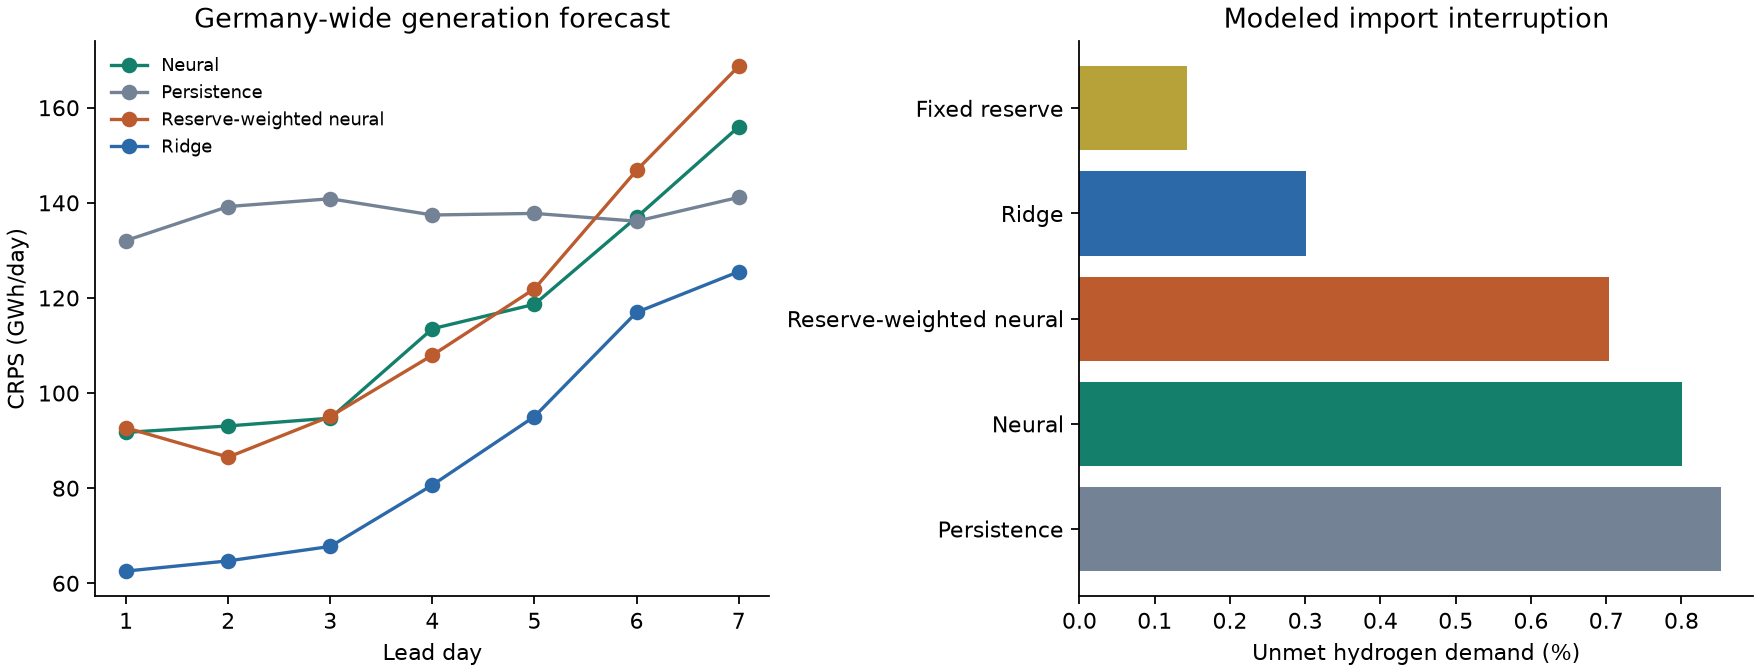
\includegraphics[width=\linewidth]{../report/backtest.png}
\caption{Forecast distribution accuracy by lead day and unmet hydrogen demand during the simulated import interruption. The right panel holds the plant, delivery obligations, and link capacities fixed across the policies.}
\end{figure}
\end{document}
